% Editable report section: Introduction and Theoretical Background
\section{Introduction and Theoretical Background}
\label{sec:1}

The geometric core implements Fortune's sweep-line algorithm to construct planar Voronoi diagrams from point sites. The program maintains a balanced beach line and an event queue, handles circle-event invalidation, and builds ordered cells clipped to a bounding rectangle. Batch commands and a graphical point-entry interface provide image and machine-readable exports. A 171-test suite, independent geometric checks and a separate reference comparison check the output. The program also provides an event replay and a Delaunay overlay. This report covers the implementation and verification available on 18 November 2026; the current construction benchmark was measured on the same date, with earlier measurements retained separately. The finite-precision limits of the implementation remain important when interpreting those results.

For sites \(P=\{p_1,\ldots,p_n\}\subset\mathbb{R}^2\), the Voronoi cell of \(p_i\) contains each query \(q\) at least as close to \(p_i\) as to every other site:
\begin{equation}
  V_i=\left\{q\in\mathbb{R}^2:
  \lVert q-p_i\rVert_2\leq\lVert q-p_j\rVert_2
  \quad\text{for every }j\neq i\right\}.
  \label{eq:cell}
\end{equation}
Each comparison defines a half-plane bounded by a perpendicular bisector. Their intersection is convex and may be unbounded. A clipping rectangle makes its visible portion finite without changing ownership inside that rectangle. Sites on the boundary of the convex hull have unbounded cells; sites strictly inside the hull have bounded cells.

The straight-line dual connects two sites when their Voronoi cells share an edge of positive length. In general position, this gives the Delaunay triangulation. A finite Voronoi vertex is the centre of an empty circumcircle through the sites of its dual triangle. Four or more cocircular sites create a higher-degree Voronoi vertex, so a triangulation of the corresponding Delaunay face is not unique. This distinction matters when choosing which adjacencies represent real Voronoi edges and which are zero-length diagonals.

\begin{figure}[!htbp]
\centering
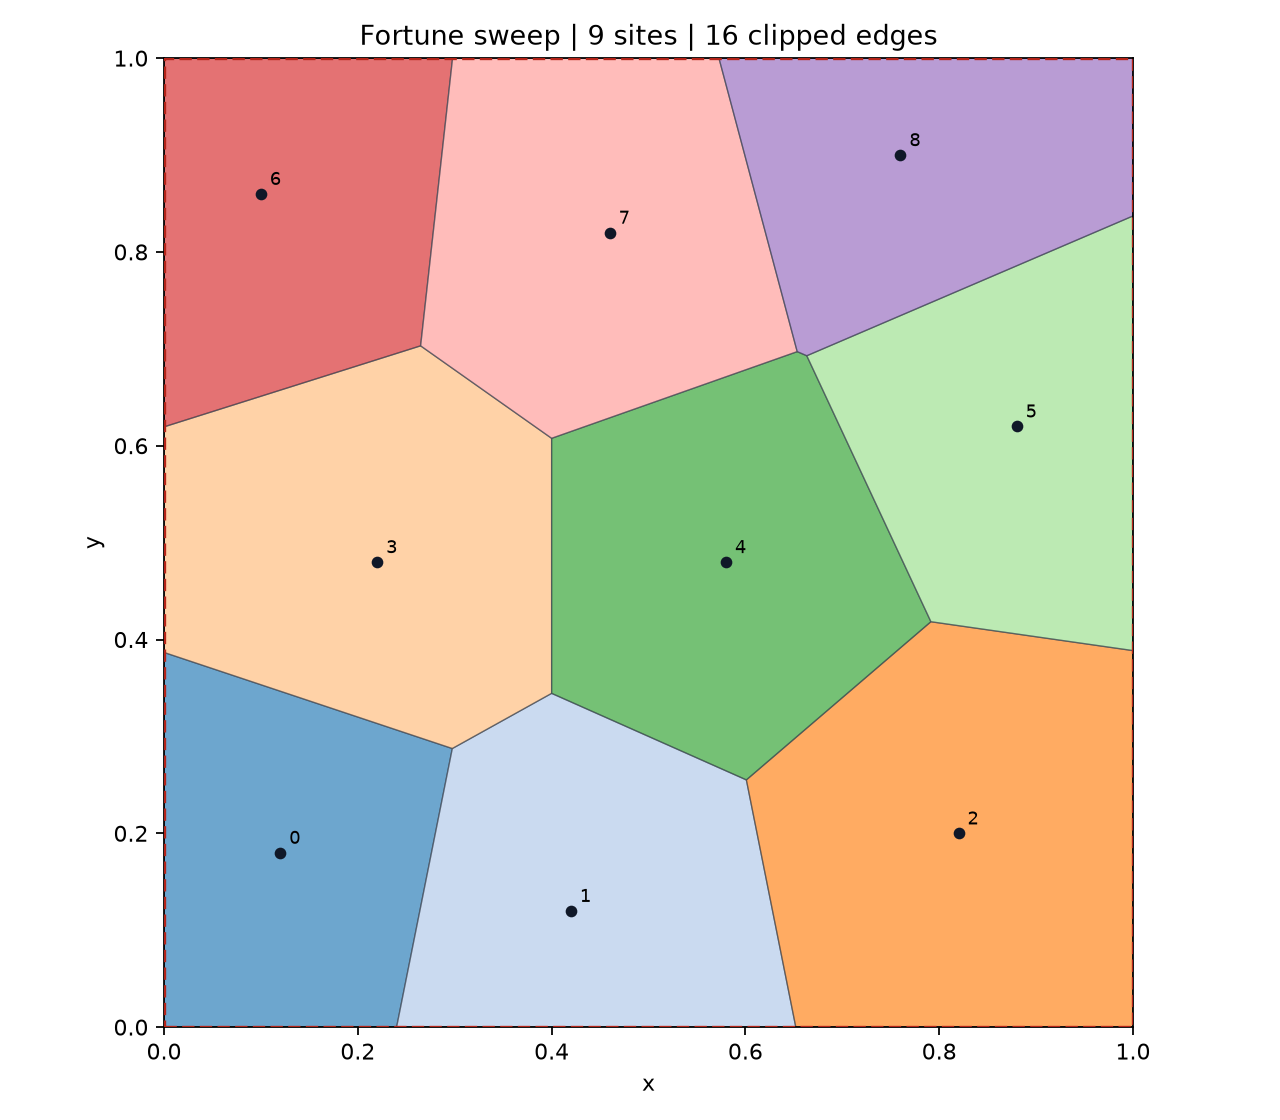
\includegraphics[width=0.86\linewidth,height=0.51\textheight,keepaspectratio]{general.png}
\caption{Nine-site Voronoi diagram clipped to the unit square.}
\label{fig:1}
\end{figure}

The dashed red rectangle is the clipping boundary. Markers and original input indices identify the sites. Shared polygon boundaries represent equal distances. The program distinguishes true circle-event vertices from corners introduced only by clipping.

\subsection{Sweep Mechanics and Degeneracies}

The directrix \(y=\ell\) moves downwards. A processed site \(p=(p_x,p_y)\), with \(p_y>\ell\), and the directrix define the parabola
\begin{equation}
  y=\frac{(x-p_x)^2}{2(p_y-\ell)}+\frac{p_y+\ell}{2}.
  \label{eq:parabola}
\end{equation}
The beach line is the lower envelope of these parabolas. Figure~\ref{fig:2} illustrates this geometric model, rather than an animation frame captured from the implementation.

\begin{figure}[!htbp]
\centering
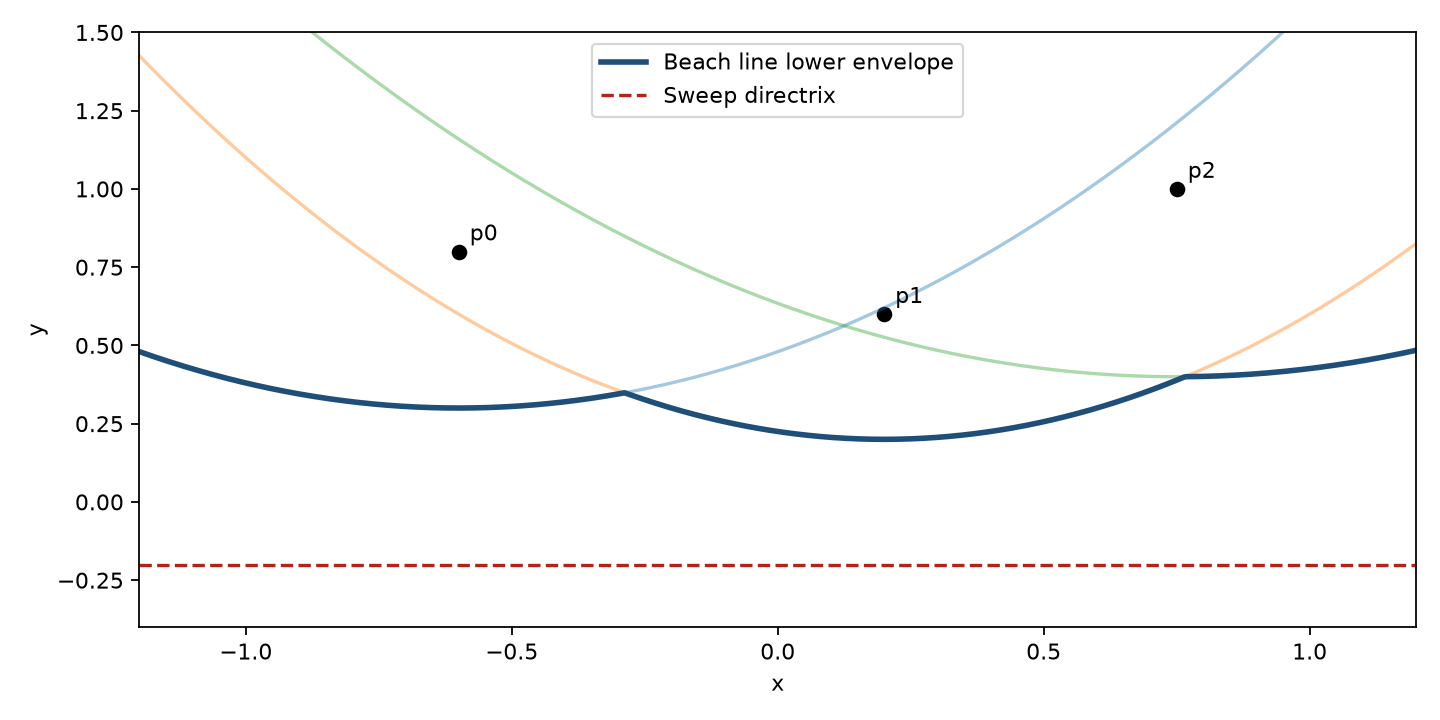
\includegraphics[width=1.0\linewidth,height=0.38\textheight,keepaspectratio]{beachline.png}
\caption{Site parabolas, sweep directrix and the beach-line lower envelope.}
\label{fig:2}
\end{figure}

A site event inserts a limiting arc and normally splits an existing arc into three. At a circle event, three consecutive arcs meet an empty circle and the middle arc disappears. For centre \(c=(c_x,c_y)\) and radius \(r\), the Voronoi vertex is \(c\), while the event height is
\begin{equation}
  \ell_{\mathrm{event}}=c_y-r.
  \label{eq:circle-event}
\end{equation}
Changes to neighbouring arcs can invalidate a pending event before it reaches the front of the queue.

Fortune's original work establishes the sweep approach and its $O(n \log n)$ time and $O(n)$ space bounds \cite{fortune1987}. The core follows the beach-line formulation and uses Python containers and mathematics. Existing Voronoi and Delaunay implementations are not used to construct the diagram.

Degeneracies need explicit policies. Exact duplicates share one cell and retain all original indices. Exactly collinear inputs reduce to consecutive one-dimensional neighbours and parallel bisectors. Equal-height events use limiting arcs. Cocircular events may share one emitted vertex. Near-coincident sites remain distinct, subject to finite-precision representation; no blanket distance threshold silently merges them.
